% !TEX root = ../../main.tex
% !TEX spellcheck = en_GB
\section{Design}
The design of the MATLAB framework is shown in \cref{fig:classbdd}.

\paragraph{The TransferFunction class} implements the \mintinline{matlab}{plotResponse(f)} method, and the  abstract method \mintinline{matlab}{transform(x)}.
\mintinline{matlab}{plotResponse(f)} plots the amplitude spectrum in the range given by the argument \mintinline{matlab}{f}.
It uses the implemented, by any subclass, \mintinline{matlab}{transform(x)} method to access the frequency response.

\begin{figure}
	\centering
	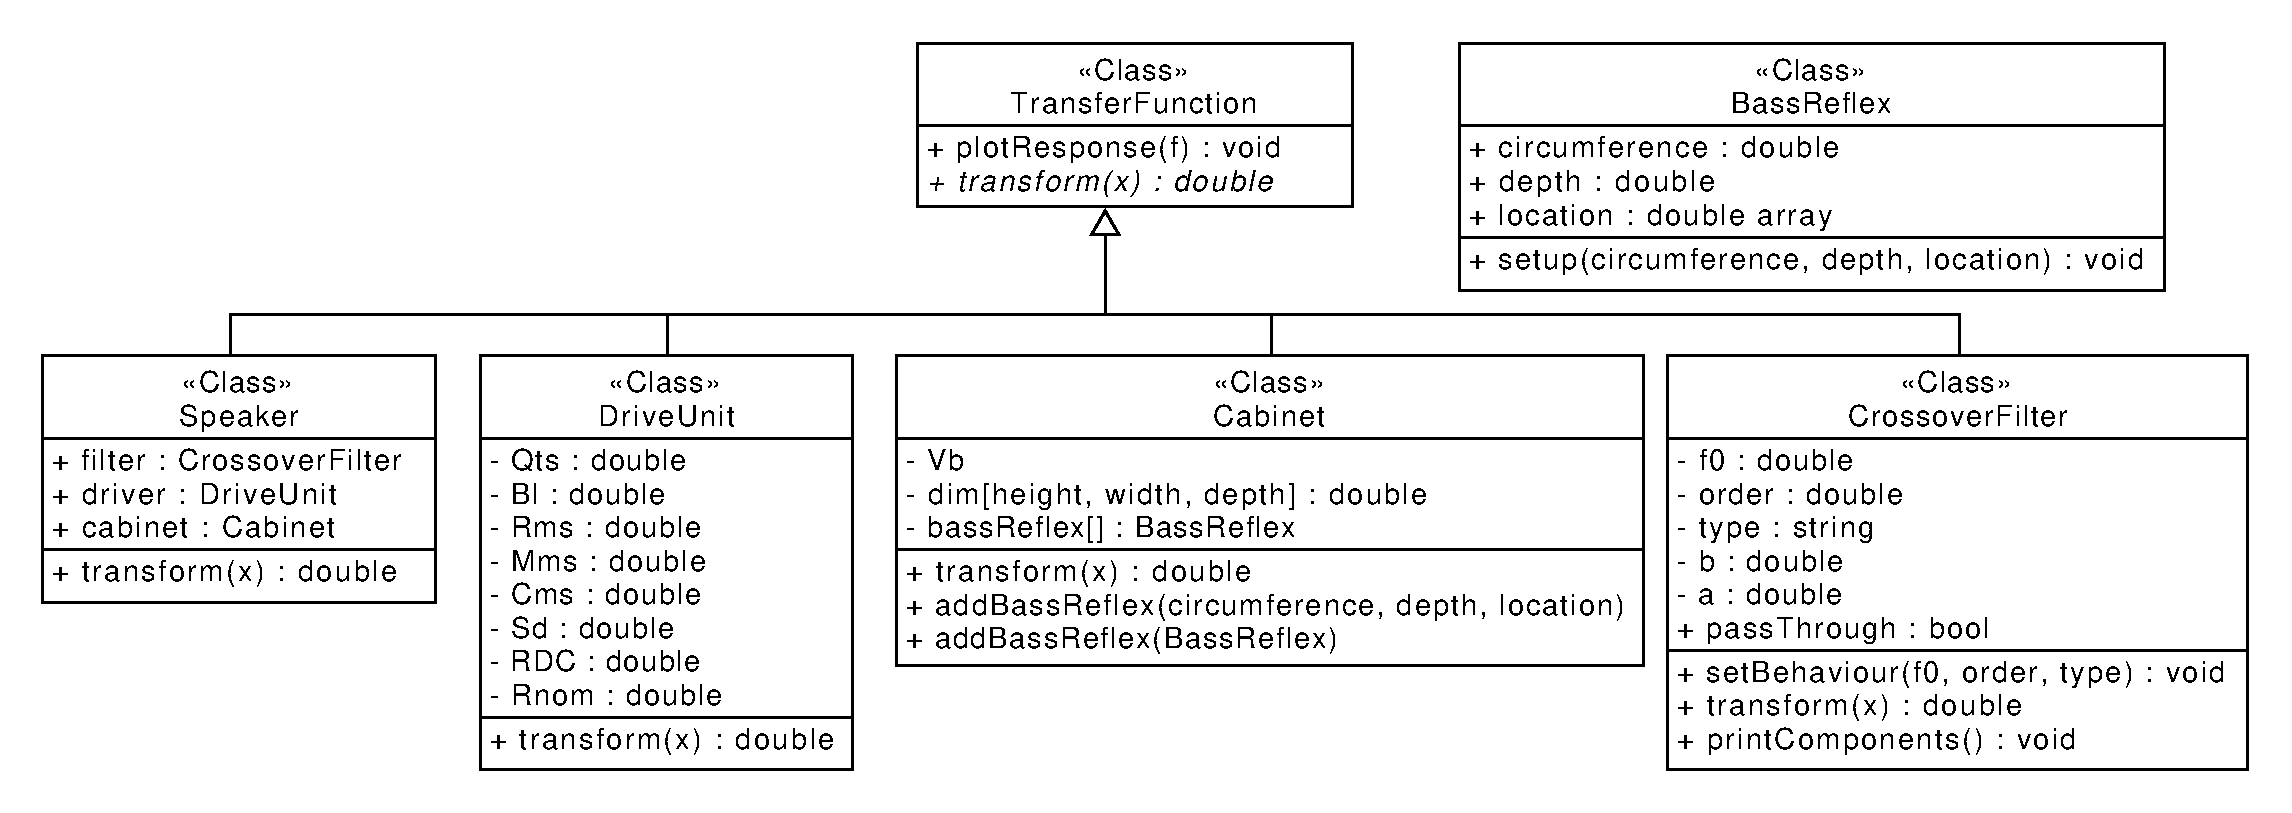
\includegraphics[width=\linewidth]{gfx/Design/Class_BDD}
	\caption{Class diagram of the MATLAB framework.}
	\label{fig:classbdd}
\end{figure}

\paragraph{The Speaker class} contains the objects necessary to calculate the transfer function for the complete speaker.
It's purpose is to collect the other units, to test them together, and to provide the frequency response to compare with the measured response.

\paragraph{The DriveUnit class}